The previous chapter introduced a method for adapting dynamics when some regions of the source and target dynamics are similar and others are not. This method allowed us to adapt a dynamics model and learn reliability in the real world. This removed the need for specialized methods for collecting real-world training data from specific regions of dynamics.

However, for all the dual-arm DOO manipulation experiments thus far, we have assumed the robot is already grasping the object, and that these grasps cannot change during the manipulation. This assumption severely limits the tasks we can do, and in some cases makes the manipulation slow compared to an approach that allows regrasping. This chapter begins to relax this assumption and use regrasping. Although I am not the first to consider regrasping deformable objects (see Section \ref{Proposed:sec:related_work} for related work), there has been little attention devoted to regrasping DOOs, and prior methods are not widely applicable to different robot morphologies or tasks. Using the proposed method, I enable robots to re-grasp when stuck, enabling new tasks and increasing robustness.

\section{Introduction}

Manipulation planning for deformable one-dimensional objects (DOOs) like ropes and cables is challenging due to the high-dimensional state representation of these objects and the cost of simulating their motion. Furthermore, most tasks benefit from multiple arms to control DOO shape and avoid becoming tangled with the environment. Therefore, the planner needs to consider the DOO, the arms manipulating it, and the environment. A task and motion planning (TAMP) approach to this problem would decompose planning into a grasp selection problem and a motion planning problem for the DOO given a specific grasp, as in \cite{RitaCableRouting,Nair2017,CFM}. However, the DOO planning problems are often expensive to solve. To reduce the space of grasps we need to search, we borrow the idea of a \textit{signature} from the field of topology.

\begin{figure}
    \centering
    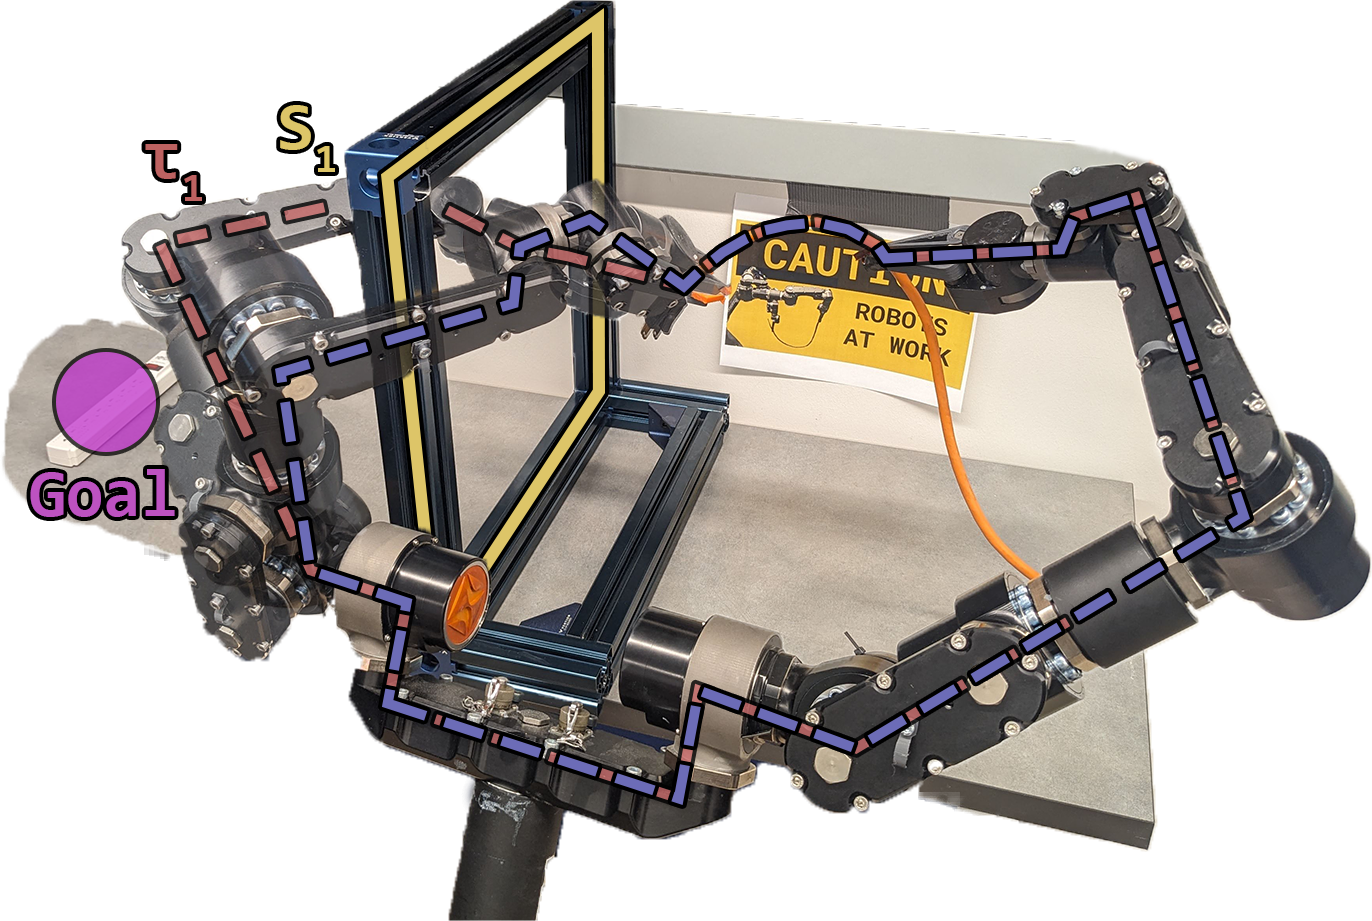
\includegraphics[width=0.8\linewidth]{Chap5/images/real_robot.png}
    \caption{Annotated image of our real world cable threading setup. The red dashed line shows a grasp loop $\tau_1$ that is linked with the skeleton $\skel_1$. The blue grasp loop is not linked with $\skel_1$. This distinction is captured by the proposed \signature{} and is used in planning.}
    \label{fig:titleFig}
\end{figure}

To explain what this signature represents, consider how the robot should grasp the tip of the cable in Figure \ref{fig:titleFig}. By grasping we form a loop, which we call a \textit{grasp loop} and show as blue and red dashed lines in Figure \ref{fig:titleFig}. It is possible to grasp either around the left side or the right side of the frame, but these two grasps are categorically different in that we cannot smoothly deform from one to the other without breaking the grasp or the frame. The frame also forms a loop, called an obstacle loop. When grasping from the left (red), these two loops are linked, but when grasping from the right (blue) they are not. Our key insight is that the robot, DOO, and environment form a \textit{graph of grasp loops} and we can use this graph to construct a signature, \signature{}, which captures topological information relevant for planning. To be clear, we do not address knots in the DOO. Our work is complimentary to work on tying or untying knots \cite{WakamatsuKnots2005, Saha07, UntanglingFull, WeifuKnots}.

The main contribution of this chapter is the \signature{} which compactly represents the topology of both the object and the arms manipulating it. We claim this signature is applicable to many systems and is useful for manipulation planning. Figure \ref{fig:examples} shows three examples where we demonstrate planning, and two more examples where the \signature{} may be useful. In simulation, we show that methods using the \signature{} outperform baselines and ablations which search for grasps without using topological information. Finally, we demonstrate a threading and point reaching task on a physical robot. Videos and animations can be found on our Project Website\footnote{\href{https://sites.google.com/view/doo-manipulation-signature/home}{https://sites.google.com/view/doo-manipulation-signature/home}}.

In the remainder of this chapter, we first review related work and then define the \signature{}. Next, we describe a method for DOO manipulation that demonstrates the utility of the \signature{}. Section \ref{chap5:sec:applications} describes how this method can be applied in three environments, which we call Pulling, Untangling, and Threading. We conclude with a brief discussion of our real world demonstration of the Threading task, which is depicted in Figure \ref{fig:titleFig}.

\section[Defining the signature]{Defining the \signature{}}
\label{sec:defHomotopy}

\begin{figure}
    \centering
    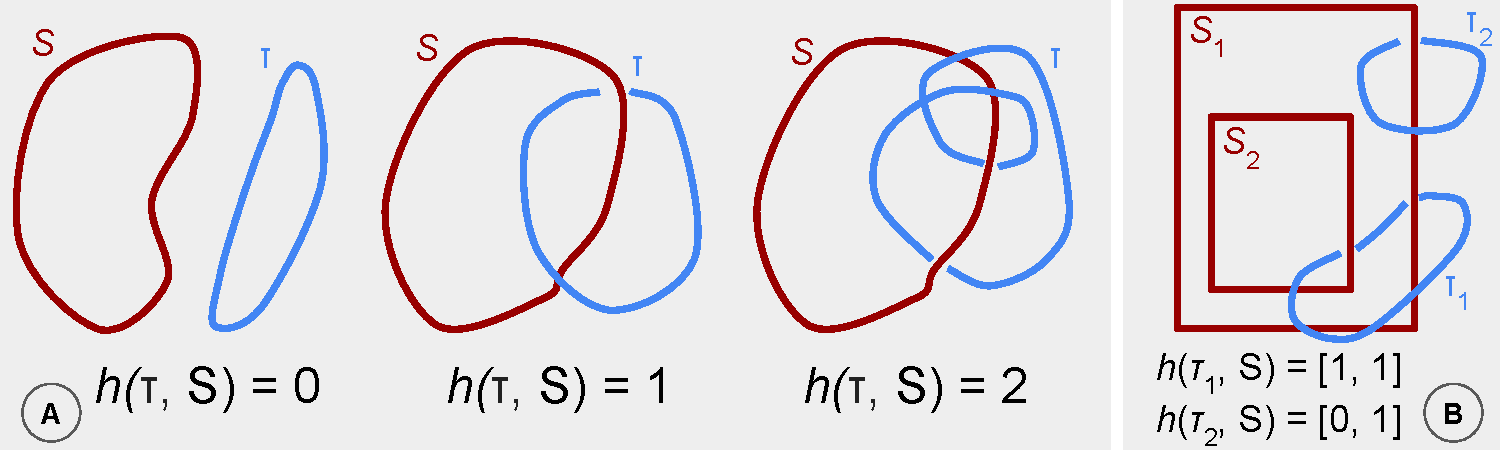
\includegraphics[width=\linewidth]{Chap5/images/simple_h.pdf}
    \caption{(A) Illustration of the h-signature for a loop representing the robot and DOO (blue) and a loop representing an obstacle (solid red). (B) Two examples of the h-signature for a skeleton with two obstacle loops $S_1$ and $S_2$.}
    \label{fig:simple_h}
\end{figure}

\subsection{Preliminaries}

We primarily use notation that is consistent with \cite{Bhattacharya11}. We call a closed one-dimensional curve in 3D a \textit{loop}. The environment is assumed to be decomposed into a \textit{skeleton} made up of multiple \textit{obstacle loops} $\skels = \{\skel_1,\dots,\skel_n\}$. Each obstacle loop is made up of line segments $\skel_i=\{\textbf{s}_i^1,\dots,\textbf{s}_i^{n_i}\}$. An example environment and corresponding skeleton is shown in Figure \ref{fig:constructingSignature}. In practice, the skeleton can either be specified manually or computed automatically from a medial axis transform of a mesh or pointcloud of the environment.

\cite{Bhattacharya11} plans paths that are in a given homotopy class or avoid a certain homotopy class. They compare two paths by considering the homotopy class of the closed loop $\tau$ formed by joining the two paths at their shared start and end points. For a path loop $\tau$ and an obstacle loop $\skel$, \cite{Bhattacharya11} defines the h-signature $h(\tau, \skel) \in \mathbb{Z}$, which counts the number of times $\tau$ passes through $\skel$. The sign of $h$ in this case is determined by the direction of $\tau$. The h-signature can be extended to a list of the h-signatures with respect to each obstacle loop in the skeleton $h(\tau, \skels)) = [h(\tau,\skel_1), \dots,h(\tau,\skel_n)]$. These cases are illustrated in Figure \ref{fig:simple_h}. The equation for computing $h(\tau,\skel)$ is reproduced from \cite{Bhattacharya11}. The point $\sk_i^{j'}$ is the point that follows $\sk_i^j$, and $r$ is a point on the loop $\tau$. The integration over $\tau$ is done numerically.

\begin{equation}
\label{eq:hsig}
\begin{split}
    h(\tau,\skel) = \frac{1}{4\pi} \int_{\tau}\sum_{j=1}^{n_i}\Phi(\sk_i^j,\sk_i^{j'}, r) \Delta r \\
    \Phi(\sk_i^j,\sk_i^{j'}, r) = \frac{1}{||d||^2} \Big( \frac{d\times p'}{||p'||} - \frac{d \times p}{||p||} \Big) \\
    p=\sk_i^j-r,\quad p'=\sk_i^{j'},\quad d=\frac{(\sk_i^{j'}-\sk_i^j)\times(p\times p')}{||\sk_i^{j'} - \sk_i^j||^2}
\end{split}
\end{equation}

We take this idea but apply it to grasp loops, instead of paths. Unlike in path planning, where the direction of $\tau$ matters, we only care how or whether loops are linked. Accordingly, we assert that $h$ is always non-negative.

\subsection[Computing the signature]{Computing the \signature{}}

\begin{figure}
    \centering
    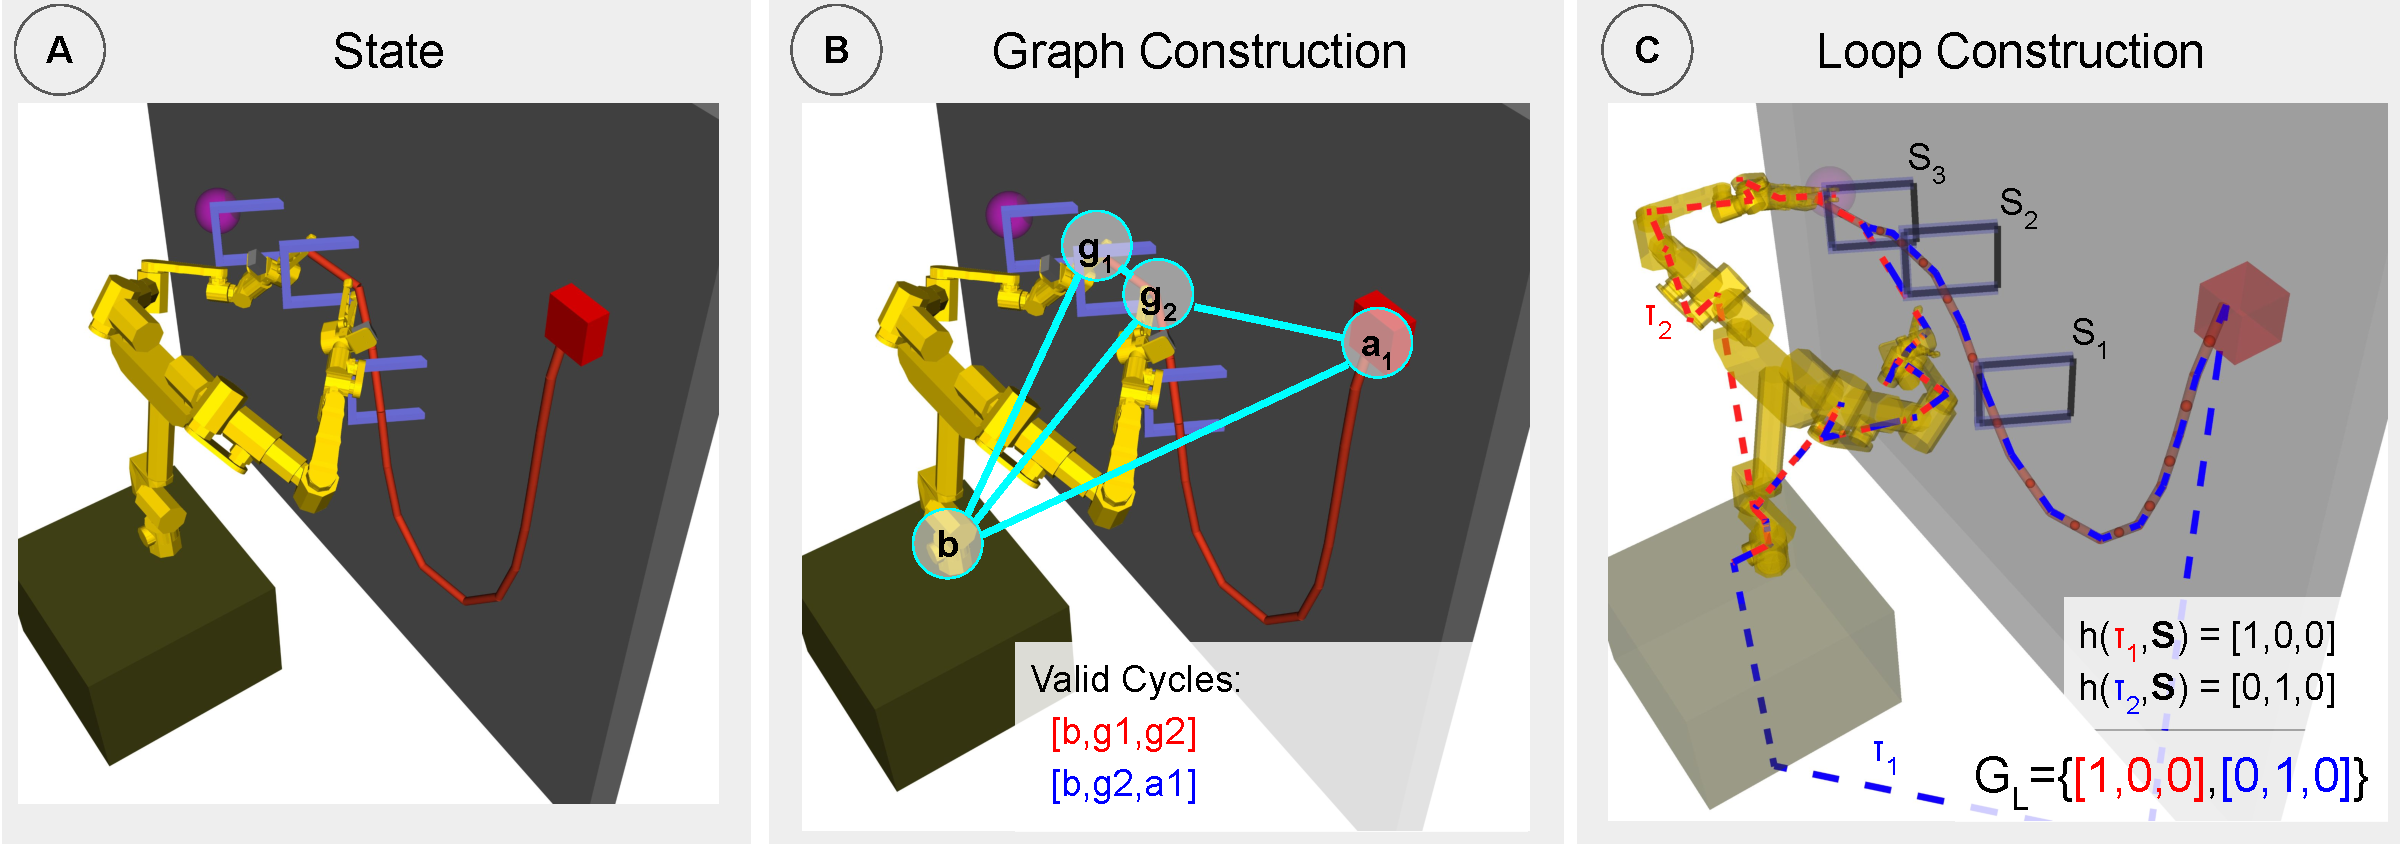
\includegraphics[width=\linewidth]{Chap5/images/alg.pdf}
    \caption{The process of constructing the \signature{}. (C) There are 2 grasp loops and 3 object loops, so the \signature{} is a set with two elements, and each element is a vector of 3 non-negative integers.}
    \label{fig:constructingSignature}
\end{figure}

The \signature{} is composed of the h-signatures $h(\tau, \skels)$ of grasp loops $\tau$ formed by the robot and  DOO. We describe the process here and in Algorithm \ref{chap5:alg:computing_signature}. The grasp loops are constructed based on a graphical model of the state $\mathcal{G}=(V,E)$ where vertices are the robot base, its grippers, and attach points, and edges are paths between them. Attach points are used to represent locations on the DOO which are fixed relative to the robot (e.g plugged into the wall or rigidly mounted on the robot itself). Figure \ref{fig:constructingSignature} illustrates how the graph construction step works. The robot base vertex is connected to all gripper and attach vertices because it connects to the grippers directly (via the robot geometry) and the attach points indirectly (via the environment). Edges connect grippers/attach points to one another if they are adjacent on the DOO. In Figure \ref{fig:constructingSignature}, the vertices $(g_1,g_2)$ are adjacent, as are $(g_2,a_1)$, but $(g_1,a_1)$ are not. In Algorithm \ref{chap5:alg:addEdges}, the function $\Adj(v_i,v_j,\state)$ checks for adjacency between $v_i$ and $v_j$ at the given state $\state$.

From $\mathcal{G}$, we extract all cycles $\cycles$ of exactly 3 distinct vertices which contain a gripper (\getValidCycles), and convert each cycle to a grasp loop $\tau$ (\getLoops). To make a grasp loop from a cycle, we concatenate the 3D paths represented by the cycles' edges. This requires a skeletonized representation of the robot geometry, which can be constructed from the kinematic tree and the origins of the links, as well as the points representing the DOO. A path between the robot base and an attach point (e.g. $(b,a_1)$ in Figure \ref{fig:constructingSignature}) can be chosen arbitrarily, as long as it is the same for all states. Cycles not containing a gripper (e.g. $(b,a_1,a_2)$) are omitted for compactness, since attach points presumably cannot be changed by the planner.

For each grasp loop, we compute the associated h-signature $h(\tau_i, \skels)$. The \signature{} of the state, denoted $\sig(\state)$, is the \textit{multiset} of the h-signatures of each grasp loop. In a multiset the order does not matter, but elements may repeat. The number of repetitions of an element is called its multiplicity. Two multisets are equivalent if their elements and multiplicities are equal. Preserving repetitions in the \signature{} allows us to represent multiple grasp loops that go through the same obstacle loop.

This may result in a grasp loop containing two grippers that has $h(\tau,\skels)=\bm{0}$ (i.e. not linked $\skels$). The red dashed grasp loop shown in Figure \ref{fig:examples} B3 is an example of this. Releasing one of the grippers does not categorically change what we can do with the object, and neither would grasping with an additional gripper right next to two already grasping. Therefore, if there is a cycle with $h(\tau,\skels)=\bm{0}$ containing two grippers, one of the grippers is removed from the graph and the process restarts from the graph construction step (Lines 7-16 in \ref{chap5:alg:computing_signature}).

This graph construction assumes a fixed base, but by constructing the graph differently, we can adapt to other scenarios. For example, we might connect drones flying together in a swarm, even though there may not be a physical connection between them. Two drones grasping the DOO simultaneously would form a loop (Fig \ref{fig:examples} E), allowing us to plan over the scene's topology.

\begin{algorithm}[t]
    \caption{Compute the \signature{}}\label{chap5:alg:computing_signature}
    \SetAlgoLined
    \DontPrintSemicolon
    \SetKwInOut{Input}{Input}
    \SetKwInOut{Output}{Output}
    
    \Input{$V, \skels, \state$}
    \Output{$\sig(\state)$}
    
   $\mathcal{G} = \addEdges(V, \state)$ \tcp*{Graph construction}
   $\cycles = \getValidCycles(\mathcal{G})$ \\
   \If{$|\cycles| = 0$}{
      \Return{$\emptyset$} \\
   }
   $\tau = \getLoops(\mathcal{G},\cycles,\state)$ \\
   \tcp{Remove empty gripper-gripper cycles (optional)}
   \For{$\tau_i \in \tau, o_i \in \cycles$}{
      \If{$h(\tau_i, \skels) = 0$}{
         \For{$v_i, v_j \in o_i$}{
            \If{$v_i,v_j$ \texttt{are gripper vertices}}{
               $V = V \setminus v_j$ \tcp*{choice of $v_j$ or $v_i$ is arbitrary}
               \textbf{goto 1} \texttt{Graph construction} \\
            }
         }
      }
   }
   \tcp{Compute final \signature{}}
   $\sig(\state) = \texttt{MultiSet}\{h(\tau_i, \skels) | \tau_i \in \tau\}$ \\
   \Return{$\sig(\state)$}
\end{algorithm}

\begin{algorithm}
    \caption{\addEdges}\label{chap5:alg:addEdges}
    \SetAlgoLined
    \DontPrintSemicolon
    \SetKwInOut{Input}{Input}
    \SetKwInOut{Output}{Output}
    
    \Input{$V, \state$}
    \Output{$\mathcal{G}$}
    
    $E = \emptyset$ \\
    \For{$v_i \in V$}{
        \For{$v_j \in V$}{
            \tcp{Skip invlid edges}
            \If{$v_i = v_j$}{
                \texttt{continue}
            }
            \ElseIf{$\neg\Adj(v_i,v_j,\state)$}{
                \texttt{continue}
            }
            $E = E \cup (v_i,v_j)$ \tcp*{Add the edge}
        }
    }
    \Return{$E$}
\end{algorithm}

\subsection{Computational Complexity}

The complexity of computing the \signature{} can be written in Big-O notation based on the number of skeletons $n_s$, number of line segments in the skeleton $l_s$, arms and/or attach points $n_a$, and the length of the arms and/or DOO $l_a$. In the base case of $n_a=2$, the graph has 3 vertices and at most cycle of length 3. And adding another vertex adds at most one cycle, so in the worst case $n_a$ arms/attach points create $n_a-1$ loops. Each cycle (loop) is compared with each skeleton, and the number of comparisons scales linearly with both the number of line segments and the length of the loop, giving a total complexity of $O\big((n_a-1) n_s l_s l_a\big)$. Our Python implementation using the NetworkX library \cite{NetworkX} for computing the \signature{} for a state takes $\leq$10ms in all environments.
\section{Illustrative Examples}

\begin{figure*}
    \centering
    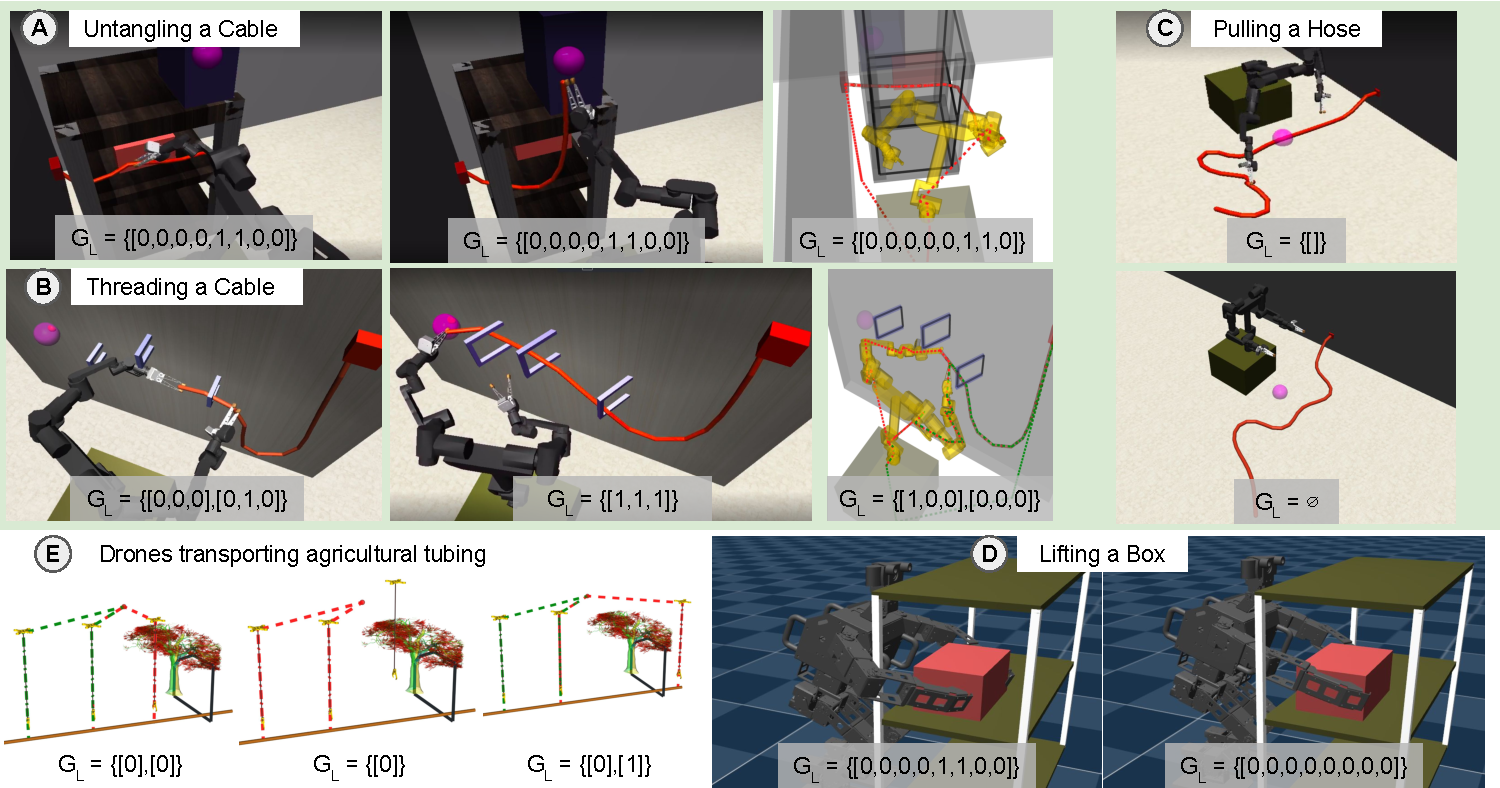
\includegraphics[width=\linewidth]{Chap5/images/examples.pdf}
    \caption{Example scenes and their $\sig$ values. The Panel in green shows environments where we use the \signature{} in planning. Panels D and E are additional examples where the \signature{} may be useful.}
    \label{fig:examples}
\end{figure*}

Figure \ref{fig:examples} shows a variety of robotic systems for which we can compute the \signature{}. The upper group show environments where we apply our planning methods. The lower group are examples where we believe the \signature{} would be useful, but do not conduct evaluations. In panel A, the second and third images show how the signature is invariant to smooth deformations, such as a change in object shape or sliding the arm along the DOO. The drones example in section C shows how we can create virtual connections between objects which are not physically connected. This allows the planner to distinguish between E1 and E3, in which the third drone is lifting the hose from different sides of the tree branch.
\section[DOO Manipulation with the signature]{DOO Manipulation with \signature{}}

\subsection{Problem Statement}

In this section, we define the DOO manipulation problem which our proposed planning method addresses. The state $\state=(q,o)$ contains the robot configuration and the DOO configuration. In our experiments, the robot has two 7-dof arms attached to a 2-dof torso with parallel-jaw grippers, but the \signature{} can be applied to other robot morphologies. We assume we have a complete geometric model and skeleton of the environment. When manipulating with the current grasp, the action space is joint velocities $\qvel$. We describe points on the DOO primarily by their location $\loc\in[0,1]$, where $\loc=0$ is one end of the DOO and $\loc=1$ is the other. Each location also corresponds to a point $p(\loc)\in\mathrm{R}^3$. Grasps are represented by a vector of locations $\locs=[\loc_1,\loc_2]$, one for each gripper. A set of grasp locations $\locs$ must also be paired with a collision-free motion of the robot to the new grasp locations, which may be reachable by many distinct joint configurations.

The goal of the manipulation is to bring a \textit{keypoint} $\kp$ on the DOO to a goal region with position $\goalPoint$ and radius $\goalRadius$. This is a useful skill for plugging in cables, or for using tools with an attached cable or hose, and more complex tasks like cable harnessing can be described as a sequence of these point reaching goals. Additionally, one can specify a desired \signature{} for the goal $\goalSig$. This type of DOO manipulation is complementary to tying or untying knots, which has been addressed in prior work \cite{Saha07,UntanglingFull,WeifuKnots}.

\subsection{DOO Point Reaching Method}

Algorithm \ref{alg:pointReaching} describes our method for point reaching tasks. However, the cost functions can be changed and additional checks can be included to adapt the method to other tasks. Given the current grasp, we use MPPI \cite{mppi} to find an action $\qvel$ that minimizes the goal cost $\goalCost$, shown in Eq \eqref{eq:pointReachingCost}. MPPI runs until the goal is reached or progress stops. If progress stops, we plan and execute a grasp change, and resume running MPPI. This process is repeated until the goal is reached (trial success) or for $\maxIters$ iterations (trial failure). For both MPPI and grasp planning, we model the dynamics of the robot, rope, and obstacles in MuJoCo \cite{mujoco}. 

\begin{algorithm}
    \caption{DOO Point Reaching with the \signature{}}\label{alg:pointReaching}
    \SetAlgoLined
    \DontPrintSemicolon
    \For{$i < \maxIters$}{
        $\qvel = $MPPI$(\state,\goalPoint, \goalCost)$ \\
        $\state = f(\qvel)$ \tcp*{Execute and get state}
        \If{$||\goalPoint - p(\kp)|| < \goalRadius$}{
            break \\
        }
        \If{trapped}{
            $d_0 = \min(|\locs_0-\kp|)$ \tcp*{Initial geodesic}
            $\locs^* = \planGrasp(\state, n_x, \graspCost, \kp)$ \\
            $d^* = \min(|\locs^*-\kp|)$ \\
            \If{$d^* \geq d_0$ \tcp*{Unable to grasp closer}}{
                Add $\sig(\state)$ to $\blist$ \\
                $\locs^* = \planGrasp(\state, n_x, \kp)$ \\
            }
            ExecuteGraspChange$(\locs^*)$ \\
        }
    }
\end{algorithm}

The method for determining if MPPI is trapped, called trap detection, is adapted from \cite{TAMPC}. Trap detection operates on a window of recent joint configurations $q_1,\dots,\q_T$, and computes the average one-step state difference $\bar{q} = \frac{q_T-q_1}{T}$ and keeps a running maximum of this value $\bar{q}^+$ over the trial. MPPI is considered trapped when the ratio $\frac{\bar{q}}{\bar{q}^+}$ is below a threshold (0.2-0.3 in our experiments).

The goal cost used for MPPI is shown in Equation \eqref{eq:pointReachingCost}, where the state $\state$ is used to compute the grasp locations $\locs$, grasping state $\isGrasping$, keypoint position $p(\kp)$, grasp positions $p(\locs)$, and number of contacts $\ncon$.

\begin{equation}
    \label{eq:pointReachingCost}
    \begin{split}
        \goalCost(\state,\qvel) = || p(\kp) - \goalPoint || + \alpha_1 \isGrasping \cdot || p(\locs) - \goalPoint || + \\
        \alpha_2\sqrt{\ncon} + \alpha_3 || \qvel ||
    \end{split}
\end{equation}

The first term in Eq.~\ref{eq:pointReachingCost} brings the keypoint $p(l_k)$ towards the goal $\goalPoint$. The second term provides a reward for moving the \textit{gripper} towards the goal. $\isGrasping$ is a binary vector indicating which grippers are grasping, and $\locs$ are the current grasp locations. The dot product enforces that only grasping grippers contribute to this cost term. This term is useful when the DOO is slack and the keypoint cannot be pulled directly (See Figure \ref{fig:examples} C). The third term penalizes collision between the robot and environment, based on the number of contacts $\ncon$ reported by the dynamics. Finally, the fourth term penalizes high joint velocities to encourage smooth motion. The hyperparameters $\alpha_{1,2,3}$ were selected to prioritize collision avoidance first, then bringing the keypoint to the goal.

In \planGrasp{} we sample $n_x$ grasps ($\approx$50) and choose the best one. Grasps are sampled first by choosing a strategy for each gripper. The possible strategies are \texttt{STAY}, \texttt{GRASP}, \texttt{MOVE}, or \texttt{RELEASE}. For the \texttt{GRASP} or \texttt{MOVE} strategies, we sample a location $\loc \in [0,1]$. At least one gripper must be grasping. For each candidate grasp, we simulate release and grasp dynamics using MuJoCo. Modeling grasping using friction and caging is challenging, so we instead use equality constraints between the rope and the grippers that are activated or deactivated. MoveIt \cite{MoveIt} is used to find collision-free paths to move the grippers to the desired grasp locations. The result is a candidate state $\state$ and collision free trajectory for each candidate grasp. We choose the grasp with the lowest cost according to Eq.~\ref{eq:graspCost}. With abuse of notation, we say the candidate state $\state$, change in $\state$, and grasp state $\isGrasping$ are derived from the candidate grasp locations $\locs$.
            
\begin{equation}
    \label{eq:graspCost}
    \begin{split}
    \graspCost(\locs)= \indic{}_\text{feasible} + \indic_{\blist}(\state) + \indic_{\sig}(\state, \goalSig) + \\
    \isGrasping \cdot |\locs - \kp | + \beta_1 \Delta \state
   \end{split}
\end{equation}

The first term in Eq \ref{eq:graspCost} assigns a large penalty (e.g. 100) if no collision-free path to the grasp was found. The next two terms assign a large penalty based on the \signature{} of candidate state, either for matching a blocklisted signature or for not matching the goal signature. If the task has no goal signature, this term is omitted. The fourth term encourages grasping near the keypoint, based on the geodesic distance for any grasping grippers. The final term penalizes the change in robot and DOO state. This results in shorter and faster grasps and is weighted by $\beta_1$ to be the least important term. The large penalties dominate the keypoint and state-change terms.

We use a blocklist of \signature{}'s to avoid retrying topological configurations in which we have failed to reach the goal. Blocklisting \signature{}s allows us to search for grasps that are different from previous states, which was an effective strategy in our experiments. However, we do not want to blocklist if the goal is reachable with a different grasp with the same signature. Therefore, we only blocklist if the planner cannot find any grasp with lower geodesic cost (4th term in Eq \eqref{eq:graspCost}) than the current grasp (Alg \ref{alg:pointReaching} lines 8-12). This heuristic avoids blocklisting the current \signature{} in the case that the current grasp cannot control the keypoint toward the goal. This is inspired by the idea of diminishing rigidity \cite{DiminishingRigidity}, which says that the control over a point on a deformable object decreases as the geodesic distance to the gripper increases. In the case of multiple grippers, the initial grasp locations $\locs_0$ or new grasp locations $\locs^*$ may be a list of locations, in which case we use the $\min$ when computing the geodesic distance (Alg \ref{alg:pointReaching} lines 8, 14).


\section{Applications}
\label{chap5:sec:applications}

We now describe how the above framework can be applied or adapted to DOO manipulation in three different environments, Pulling, Untangling, and Threading.

\subsection{Pulling Environment}

The Pulling environment contains a large hose attached to a wall. The scene is depicted in Figure \ref{fig:examples} C. The robot is initially not grasping the hose, and the head of the hose is out of the robot's reach. The goal region, shown as a purple sphere, is near the base of the robot on the floor. This environment requires regrasping to bring the keypoint to the goal, and demonstrates the behavior of the general method in the case where there are no skeletons, and no changes in the \signature{}.

When applying Alg \ref{alg:pointReaching} in this environment, the robot initially chooses a grasp as far down the DOO as it can reach, due to the geodesic cost term in Equation \ref{eq:graspCost}. Then, the gripper pulls towards the goal due to the second term in the MPPI cost \eqref{eq:pointReachingCost}. This brings more of the DOO within reach. When the gripper reaches the goal, the cost cannot be decreased and the controller slows to a stop. At this point, trap detection triggers regrasp planning. Since the DOO is now closer, a plan is found that reaches closer to the tip ($\kp=1$) than before. Because the grasp is closer to the tip, the current \signature{} is not blocklisted. This repeats until the grasp is close enough to the tip that it can be brought to the goal region. In the Pulling environment, our method succeeded in 25/25 trials, where each trial differs in the initial DOO configuration and the random seed used for sampling in planning.

\subsection{Untangling Environment}

\begin{table}
    \centering
    \begin{tabular}{ccccc}
        Method & Success & Wall Time (m) & Sim Time (m) \\ \hline
        \signature{} (ours) & 22/25 & 12 (5) & 1.4 (1.1) \\
        Always Blocklist & 22/25 & 14 (7) & 1.3 (1.0) \\
        No \signature{} & 10/25 & 20 (10) & 2.0 (1.3) \\
        TAMP50 & 15/25 & 142 (116) & 2.4 (1.7) \\
        TAMP5 & 9/25 & 34 (22) & 1.8 (1.2) \\
    \end{tabular}
    \caption{Results in the Untangle environment. Times in minutes are for the completion of the task, where Sim Time does not include planning time. Standard deviations are given in parentheses.}
    \label{tab:point_reaching}
\end{table}

The Untangle environment resembles a computer rack with a cable that needs to be plugged in. The scene is depicted in Figure \ref{fig:examples} A. One end of the DOO is fixed to the environment (e.g. plugged in elsewhere), and the robot is initially grasping some other location on the DOO. The robot often needs to regrasp several times in order to reach the goal. Unlike in the Pulling environment, the \signature{} can take on many different values depending on the configuration of the DOO and the grasp configuration. This demonstrates the utility of the \signature{} in planning when there is no goal \signature{}.

We evaluate Alg \ref{alg:pointReaching} on this task, and compare to an ablation that omits the two terms using the \signature{} from Eq \ref{eq:graspCost}. We call this method \textit{No \signature{}}. This often results in greedy re-grasping of the keypoint. We also evaluate a version called \textit{Always Blocklist}, where we blocklist the current \signature{} every time a trap is detected. Finally, we compare our proposed method to a method inspired by task and motion planning (TAMP), where $H$ additional steps of MPPI are simulated for each candidate grasp during planning and the final goal cost is used in place of cost terms relying on the \signature{}. We test two versions of this method with $H=5$ and $H=50$. Success rates and trial times are shown in Table \ref{tab:point_reaching}. Trials vary in the initial configuration of the robot, grasp location, DOO configuration, in the size of the computer rack, and in the location of the goal.

Methods using the \signature{} have the highest success rates and are faster than alternatives. \textit{Always Blocklist} has an equivalent success rate as the full proposed method, but prematurely abandons grasps that would lead to reaching the goal. Our method and the \textit{Always Blocklist} method each failed in 3 trials by trying too many unsuccessful grasps before $\maxIters$ was reached. The \textit{No \signature{}} ablation and both TAMP methods usually fail by greedily trying to grasp the keypoint. Without a very long horizon or the \signature{}, the planner often grasps with configurations that make reaching the goal impossible. The longer horizon used in $H=50$ helps alleviate this issue but is insufficient in many cases while also causing a 10x increase in planning time.

\subsection{Threading Environment} 

In the Threading environment, the objective is for the robot to thread the DOO through a series of fixtures in a specified order (e.g. "fixture 1, then fixture 2, then fixture 3"), after which it should bring the keypoint to a goal region. The threading is described by a series of goal signatures $\sig_1,\dots,\sig_N$. This skill could be applied to installing cable harnesses in a car or electrical wiring in a building. One end of the DOO is fixed to the environment, and the robot is initially grasping some other location on the DOO. This environment is depicted in Figure \ref{fig:examples} B.

\begin{algorithm}[t]
    \caption{DOO Threading with the \signature{}}\label{alg:threading}
    \SetAlgoLined
    \DontPrintSemicolon
    $j = 1$ \tcp*{Threading subgoal index}
    \For{$i < \maxIters$}{
        \eIf{$j<N$ \tcp*{threading subgoals}}{
           $\qvel = $MPPI$(\state,\sig_j, \goalCost)$ \\
           $\state = f(\qvel)$ \tcp*{Execute and get state}
            \If{{\color{green}disc penetrated}}{
             $\locs^* = \planGrasp(\state, n_x,\graspCost, {\color{green}1})$ \\
                \If{{\color{green} $\sig(\locs^*) == \sig_j$}}{
                    ExecuteGraspChange$(\locs^*)$ \\
                }
            }
            \If{trapped}{
               $\locs^* = \planGrasp(\state, n_x, \graspCost, {\color{green}\loc-0.05})$ \\
                ExecuteGraspChange$(\locs^*)$ \\
            }
            \If{{\color{green} $\sig(\state) == \sig_j$}}{
                $j = j + 1$ \tcp*{next subgoal}
            }
        }{
            $\qvel = $MPPI$(\state,\goalPoint, \goalCost)$ \\
            $\state = f(\qvel)$ \tcp*{Execute and get state}
            \If{$\goalPoint - p(\kp) < \goalRadius$}{
                 break \\
            }
        }
    }
\end{algorithm}

We extend Alg \ref{alg:pointReaching} for this task in several ways. First, we run it iteratively, looping over each of the three threading subgoals, then finally for the point reaching subgoal. Second, when using MPPI to reach a threading subgoal, we augment Eq \eqref{eq:pointReachingCost} with the magnetic-field cost proposed in \cite{Weifu}. This uses the formula $\sum_{j=1}^{n_i}\Phi(\sk_i^j,\sk_i^{j'}, r)$ from in Equation \eqref{eq:hsig} for the direction of the magnetic field, but where $r$ is the keypoint of the DOO. This causes the keypoint to follow virtual magnetic field lines through the fixture in the specified direction. Third, if a threading subgoal is reached, and the planner returns a grasp which does not match $\goalSig$, we reject it and continue running MPPI to push the cable further through the fixture. This happens when there is no feasible grasp matching $\goalSig$ due to obstacles or reachability issues. Furthermore, we also check $\goalSig$ after executing the grasp to ensure that any deviations that occurred when executing the grasp plan do not change the \signature{}. To check when a threading subgoal is reached, we use the disc penetration check from \cite{Weifu}. The goal signatures $\sig_1,\dots,\sig_N$ are used in the grasp planning (3rd term in Eq \eqref{eq:graspCost}), but the blocklist is not. Grasp sampling is restricted to alternating single-gripper grasps, which speeds up grasp planning. The keypoint location for grasp planning is also restricted. It is chosen to be the tip ($\kp=1$) when a threading subgoal is reached, and further down the DOO than the current grasp when stuck ($\kp=\loc-0.05$). The full Threading algorithm is shown in Alg \ref{alg:threading}, with the key differences highlighted in green.
We compare our proposed method to the TAMP5 method described previously. In this environment, the TAMP method often chooses grasps that correctly thread through fixtures 1 and 2, because those grasps allow immediate progress towards the next subgoal. However, it often grasps incorrectly on fixture 3, which requires the robot to first reach further around and results in less immediate progress towards the next subgoal. We also adapted the method in \cite{Weifu} from a single floating gripper to our dual arm robot. As in our method, we use alternating single-gripper grasps. Instead of the more general trap detection method we use, this baseline checks the distance between the gripper and the fixture being threaded. This baseline fails similarly to the TAMP5 method, but additionally fails when MPPI is trapped but is outside the distance-to-fixture threshold. Success rates and trial times are shown in Table \ref{tab:threading}. Trials vary in the initial configuration of the robot, grasp location, DOO configuration, and in the positions of the fixtures. In the trials in which our method failed to complete the task, MPPI reached a joint configuration with one arm that prevented the other arm from grasping the DOO at or near the tip, as required by our method. This means the robot remained stuck until $\maxIters$ was reached.

\begin{table}
    \centering
    \begin{tabular}{cccc}
    % NOTE: these results came from the combination of:
    % threading_ours_v5
    % threading_tamp_v5
    % threading_wang_v5
    % threading_ours_v4
    % threading_wang_v4
    % threading_tamp5_v4
        Method & Success & Wall Time (m) & Sim Time (m) \\ \hline
        \signature{} & 42/50 & 8 (2) & 1.3 (0.4) \\
        TAMP5 & 21/50 & 17 (3) & 1.3 (0.6) \\
        Wang et al. \cite{Weifu} & 12/50 & 8 (3) & 1.0 (0.8) \\
    \end{tabular}
    \caption{Results on the Threading task.}
    \label{tab:threading}
\end{table}

%%%%%%%%%%%%%%%%%%%%%%%%%%%%%%%%%%%%%%%%%%%%%%%%%%%%%%%%%%%%%%%%%%%%%%%%%%%%%%%%%%%%%%%%%%%%%%%%%%%%%%%%%%%%%%%%%%%

\subsection{Real World Threading}

We demonstrate a simplified version of the Threading task in the real world, as depicted in Figure \ref{fig:titleFig}. This shows the applicability of the proposed methods in the presence of significant calibration, perception, and dynamics modeling errors. We use CDCPD2 \cite{CDCPD2} to track the DOO and visual servoing from in-hand cameras to guide grasping. The environment geometry is specified manually, and the simulation dynamics were tuned to match the real world setup as closely as possible for the particular setup.
\section{Conclusion}

In this paper, we proposed the \signature{} which describes the topology of closed loops formed by grasping the DOO with respect to closed loops formed by stationary objects in the environment. Our \signature{} builds on the h-signature proposed in prior work on topological path planning. Furthermore, we describe an algorithm for manipulating DOOs that plans grasps based on the proposed \signature{}. In our experiments, we find that using the \signature{} improves task success and reduces planning times compared to a task and motion-planning method. Finally, we use the method to thread a cable and bring it to a goal region on a real robot.
